\chapter{Adding Entries}
So, there are a number of ways to enter information into the database, below we will discuss each one in turn.
\section{Albums}
\label{sect:albums}
We add data by adding albums.  Select the \textit{\textbf{Add Album}} button 
as shown in Figure \ref{fig:albumbutton2}.
\begin{figure}[h]
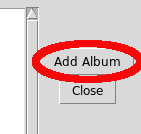
\includegraphics[scale=1]{albumButton2.png}
\caption{Add Album}
\label{fig:albumbutton2}
\end{figure}
You should see the \textit{\textbf{New Album}} screen (Figure \ref{fig:addemptyalbum}).
\begin{figure}[h]
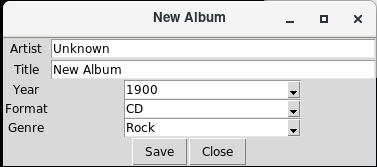
\includegraphics[scale=1]{addAlbum.png}
\caption{Add Album}
\label{fig:addemptyalbum}
\end{figure}
This is the key to entering all the data into the database.

\subsection{The first entry}
So, let's get on and enter that first album into our new database.  You will have noticed, from Figure \ref{fig:addemptyalbum}, that some details have been pre-populated.  When a new database is created the \textit{\textbf{Format}} table is populated with an entry \textit{\textbf{CD}}, and the
\textit{\textbf{Genre}} table is populated with an entry \textit{\textbf{Rock}} \footnote{See Part II, Tables for  full details of the Database structure.}, as a convenience to get things started.

\section{Artists}
\section{CSV}
\label{sect:csv}